\documentclass[tikz]{standalone}
\usepackage{bm}
\begin{document}
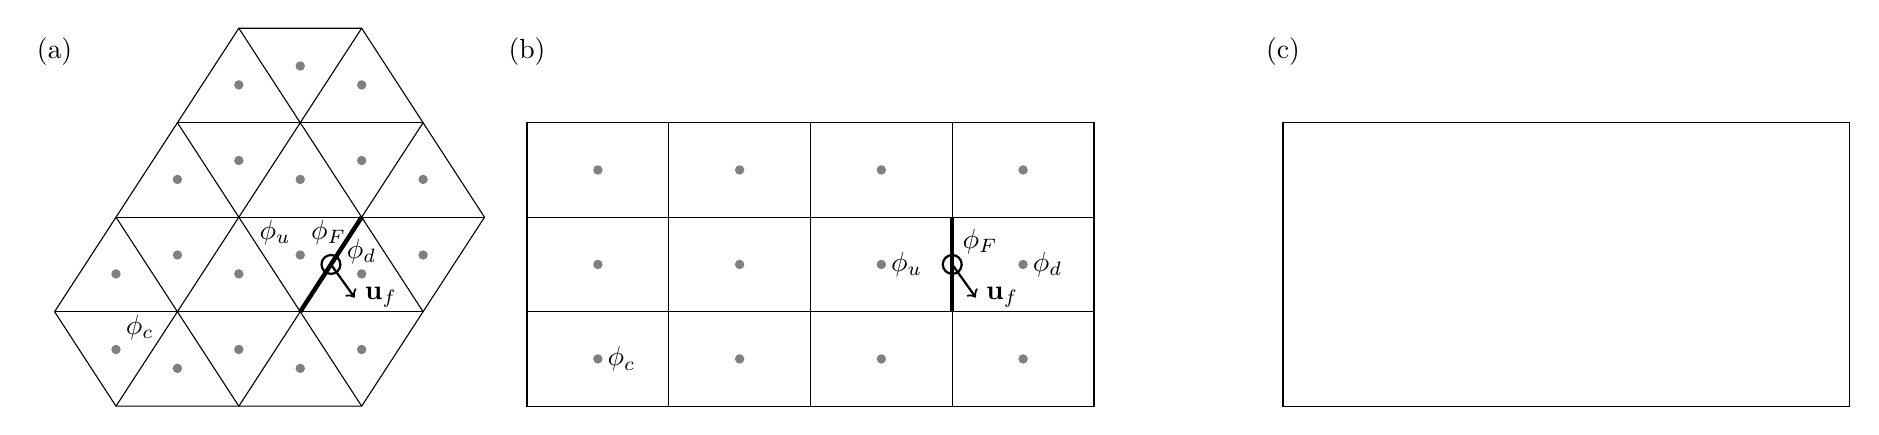
\begin{tikzpicture}[
  scale=0.6,
  cpnt/.style={fill=gray},
]

\begin{scope}
	\node [above] at (0,7) {(a)};
	\draw (0,2) -- (1.3,0) -- (6.5,0) -- (9.1,4) -- (6.5,8) -- (3.9,8) -- (0,2);

	\draw (0,2) -- (7.8,2);
	\draw (1.3,4) -- (9.1,4);
	\draw (2.6,6) -- (7.8,6);

	\draw (1.3,0) -- (6.5,8);
	\draw (3.9,0) -- (7.8,6);
	\draw (1.3,4) -- (3.9,0);
	\draw (2.6,6) -- (6.5,0);
	\draw (3.9,8) -- (7.8,2);

	\path [cpnt] (1.3,1.2) circle [radius=0.1] node [anchor=south west] {$\phi_c$};
	\path [cpnt] (2.6,0.8) circle [radius=0.1];
	\path [cpnt] (3.9,1.2) circle [radius=0.1];
	\path [cpnt] (5.2,0.8) circle [radius=0.1];
	\path [cpnt] (6.5,1.2) circle [radius=0.1];

	\path [cpnt] (1.3,2.8) circle [radius=0.1];
	\path [cpnt] (2.6,3.2) circle [radius=0.1];
	\path [cpnt] (3.9,2.8) circle [radius=0.1];
	\path [cpnt] (5.2,3.2) circle [radius=0.1] node [anchor=south east] {$\phi_u$};
	\path [cpnt] (6.5,2.8) circle [radius=0.1] node [above] {$\phi_d$};
	\path [cpnt] (7.8,3.2) circle [radius=0.1];

	\path [cpnt] (2.6,4.8) circle [radius=0.1];
	\path [cpnt] (3.9,5.2) circle [radius=0.1];
	\path [cpnt] (5.2,4.8) circle [radius=0.1];
	\path [cpnt] (6.5,5.2) circle [radius=0.1];
	\path [cpnt] (7.8,4.8) circle [radius=0.1];

	\path [cpnt] (3.9,6.8) circle [radius=0.1];
	\path [cpnt] (5.2,7.2) circle [radius=0.1];
	\path [cpnt] (6.5,6.8) circle [radius=0.1];

	\draw [ultra thick] (5.2,2) -- (6.5,4);
	\draw [thick] (5.85,3) circle [radius=0.2];
	\node at (5.8,3.2) [above] {$\phi_F$};
	\draw [thick, ->] (5.85,3) -- (6.35,2.3) node [anchor=west] {$\mathbf{u}_f$};
\end{scope}

\begin{scope}[shift={(10,0)}]
	\node [above] at (0,7) {(b)};
	\draw (0,0) rectangle (12,6);
	\draw (0,2) -- (12,2);
	\draw (0,4) -- (12,4);
	\draw (0,0) -- (0,6);
	\draw (3,0) -- (3,6);
	\draw (6,0) -- (6,6);
	\draw (9,0) -- (9,6);

	\draw [ultra thick] (9,2) -- (9,4);
	\draw [thick] (9,3) circle [radius=0.2] node [anchor=south west] {$\phi_F$};
	\draw [thick, ->] (9,3) -- (9.5,2.3) node [anchor=west] {$\mathbf{u}_f$};

	\path [cpnt] (1.5,1) circle [radius=0.1] node [right] {$\phi_c$};
	\path [cpnt] (1.5,3) circle [radius=0.1];
	\path [cpnt] (1.5,5) circle [radius=0.1];

	\path [cpnt] (4.5,1) circle [radius=0.1];
	\path [cpnt] (4.5,3) circle [radius=0.1];
	\path [cpnt] (4.5,5) circle [radius=0.1];

	\path [cpnt] (7.5,1) circle [radius=0.1];
	\path [cpnt] (7.5,3) circle [radius=0.1] node [right] {$\phi_u$};
	\path [cpnt] (7.5,5) circle [radius=0.1];

	\path [cpnt] (10.5,1) circle [radius=0.1];
	\path [cpnt] (10.5,3) circle [radius=0.1] node [right] {$\phi_d$};
	\path [cpnt] (10.5,5) circle [radius=0.1];
\end{scope}

\begin{scope}[shift={(26,0)}]
	\node [above] at (0,7) {(c)};
	\draw (0,0) rectangle (12,6);
\end{scope}

\end{tikzpicture}
\end{document}
